\section{Dreidimensionale Richtungsbestimmung}
\subsection{Erweiterung der Theorie}
Um die Richtungsbestimmung dann auf drei Dimensionen zu erweitern, müssen zuerst die Ortsvektoren der Mikrofone und der Schallquelle auf drei Dimensionen erweitert werden:
\begin{equation}
    \vec{m}_i = \begin{pmatrix}
        m_{ix} \\
        m_{iy} \\
        m_{iz}
    \end{pmatrix} \quad\quad
    \vec{s} = \begin{pmatrix}
        {s_x} \\
        {s_y} \\
        {s_z}
    \end{pmatrix}
\end{equation}
Mit den angepassten Ortsvektoren erhält man eine neue Formel für die Abstandsberechnung zwischen einem Mikrofon und der Schallquelle:
\begin{equation}
    \abs{\vec{m}_i - \vec{s}} = \sqrt{{(m_{ix} - s_x)}^2 + {(m_{iy} - s_y)}^2 + {(m_{iz} - s_z)}^2}
\end{equation}
Man erhält eine weitere Unbekannte, $m_{iz}$. Dadurch wird für die dreidimensionale Ortung ein viertes Mikrofon benötigt. Mit dem vierten Mikrofon erhält man eine dritte Gleichung, die den Gangunterschied zwischen dem ersten und dem vierten Mikrofon enthält, dadurch wird das Gleichungssystem wieder eindeutig lösbar:
\begin{gather*}
    \begin{vmatrix}
        \abs{\vec{m}_1 - \vec{s}} - \abs{\vec{m}_2 - \vec{s}} = \Delta{x_{12}} \\
        \abs{\vec{m}_1 - \vec{s}} - \abs{\vec{m}_3 - \vec{s}} = \Delta{x_{13}} \\
        \abs{\vec{m}_1 - \vec{s}} - \abs{\vec{m}_4 - \vec{s}} = \Delta{x_{14}}
    \end{vmatrix}\\
    \begin{vmatrix}
        \sqrt{{(m_{1x} - s_x)}^2 + {(m_{1y} - s_y)}^2 + {(m_{1z} - s_z)}^2} - \sqrt{{(m_{2x} - s_x)}^2 + {(m_{2y} - s_y)}^2 + {(m_{2z} - s_z)}^2} = \Delta{x_{12}} \\
        \sqrt{{(m_{1x} - s_x)}^2 + {(m_{1y} - s_y)}^2 + {(m_{1z} - s_z)}^2} - \sqrt{{(m_{3x} - s_x)}^2 + {(m_{3y} - s_y)}^2 + {(m_{3z} - s_z)}^2} = \Delta{x_{13}} \\
        \sqrt{{(m_{1x} - s_x)}^2 + {(m_{1y} - s_y)}^2 + {(m_{1z} - s_z)}^2} - \sqrt{{(m_{4x} - s_x)}^2 + {(m_{4y} - s_y)}^2 + {(m_{4z} - s_z)}^2} = \Delta{x_{14}}
    \end{vmatrix}
\end{gather*}
\subsection{Numerische Lösung des Gleichungssystems}
Schon für zwei Dimensionen ist die analytische Lösung des Gleichungssystems sehr kompliziert. Für drei Dimensionen ist die Formel der Lösung in Textform über \num{300}~Mb groß. Dadurch können wir sie nur durch Einschränkung der Mikrofon-Positionen verwenden. Um diese Einschränkung zu umgehen, lösen wir das Gleichungssystem numerisch. Dazu verwenden wir das mehrdimensionale Newtonverfahren. Hierbei gehen wir von einer Startposition $\vec{s}_0$ aus, die iterativ verbessert wird. Als Startposition haben wir das Zentrum der Mikrofone gewählt.
Für jeden weiteren Iterationsschritt $i$ erhält man ein $\vec{\Delta{s}}_i$, mit dem man die neuen Positionen für den nächsten Iterationsschritt mit $\vec{s}_{i + 1} = \vec{s}_i + \vec{\Delta{s}}_i$ erhält.
Um das Gleichungssystem mit dem Newtonverfahren zu lösen, wird es mit der Taylorentwicklung bis zur ersten Ordnung linearisiert:
\begin{gather*}
    r_{i_{ca}} = \sqrt{(m_{ix} - s_{ix})^2 + (m_{iy} - s_{iy})^2 + (m_{iz} - s_{iz})^2}\\
    \begin{vmatrix}
        \Delta{x_{12}} - r_{2_{ca}} + r_{1_{ca}} = \left(\frac{s_{ix} - m_{2x}}{r_{2_{ca}}} - \frac{s_{ix} - m_{1x}}{r_{1_{ca}}} \right) \Delta{s}_{ix} + \left(\frac{s_{iy} - m_{2y}}{r_{2_{ca}}} - \frac{s_{iy} - m_{1y}}{r_{1_{ca}}} \right)  \Delta{s}_{iy} + \left(\frac{s_{iz} - m_{2z}}{r_{2_{ca}}} - \frac{s_{iz} - m_{1z}}{r_{1_{ca}}} \right)  \Delta{s}_{iz} \\
        \Delta{x_{13}} - r_{3_{ca}} + r_{1_{ca}} = \left(\frac{s_{ix} - m_{3x}}{r_{3_{ca}}} - \frac{s_{ix} - m_{1x}}{r_{1_{ca}}} \right) \Delta{s}_{ix} + \left(\frac{s_{iy} - m_{3y}}{r_{3_{ca}}} - \frac{s_{iy} - m_{1y}}{r_{1_{ca}}} \right)  \Delta{s}_{iy} + \left(\frac{s_{iz} - m_{3z}}{r_{3_{ca}}} - \frac{s_{iz} - m_{1z}}{r_{1_{ca}}} \right)  \Delta{s}_{iz} \\
        \Delta{x_{14}} - r_{4_{ca}} + r_{1_{ca}} = \left(\frac{s_{ix} - m_{4x}}{r_{4_{ca}}} - \frac{s_{ix} - m_{1x}}{r_{1_{ca}}} \right) \Delta{s}_{ix} + \left(\frac{s_{iy} - m_{4y}}{r_{4_{ca}}} - \frac{s_{iy} - m_{1y}}{r_{1_{ca}}} \right)  \Delta{s}_{iy} + \left(\frac{s_{iz} - m_{4z}}{r_{4_{ca}}} - \frac{s_{iz} - m_{1z}}{r_{1_{ca}}} \right)  \Delta{s}_{iz} \\
    \end{vmatrix}\\
    \begin{pmatrix}
        {\Delta{s}}_{ix} \\
        {\Delta{s}}_{iy} \\
        {\Delta{s}}_{iz} \\
    \end{pmatrix}
    =
    {\begin{pmatrix}
          \frac{s_{ix} - m_{2x}}{r_{2_{ca}}} - \frac{s_{ix} - m_{1x}}{r_{1_{ca}}} & \frac{s_{iy} - m_{2y}}{r_{2_{ca}}} - \frac{s_{iy} - m_{1y}}{r_{1_{ca}}} & \frac{s_{iz} - m_{1z}}{r_{2_{ca}}} - \frac{s_{iz} - m_{1z}}{r_{1_{ca}}} \\
          \frac{s_{ix} - m_{3x}}{r_{3_{ca}}} - \frac{s_{ix} - m_{1x}}{r_{1_{ca}}} & \frac{s_{iy} - m_{3y}}{r_{3_{ca}}} - \frac{s_{iy} - m_{1y}}{r_{1_{ca}}} & \frac{s_{iz} - m_{1z}}{r_{3_{ca}}} - \frac{s_{iz} - m_{1z}}{r_{1_{ca}}} \\
          \frac{s_{ix} - m_{4x}}{r_{4_{ca}}} - \frac{s_{ix} - m_{1x}}{r_{1_{ca}}} & \frac{s_{iy} - m_{4y}}{r_{4_{ca}}} - \frac{s_{iy} - m_{1y}}{r_{1_{ca}}} & \frac{s_{iz} - m_{1z}}{r_{4_{ca}}} - \frac{s_{iz} - m_{1z}}{r_{1_{ca}}} \\
      \end{pmatrix}}^{-1}
    \cdot
    \begin{pmatrix}
        \Delta{x_{12}} - r_{2_{ca}} + r_{1_{ca}}\\
        \Delta{x_{13}} - r_{3_{ca}} + r_{1_{ca}}\\
        \Delta{x_{14}} - r_{4_{ca}} + r_{1_{ca}}
    \end{pmatrix}
\end{gather*}

Für die Berechnung der Inverse der Matrix gibt es viele verschiedene Methoden, wir benutzen die Singulärwertzerlegung, da diese verhältnismäßig numerisch stabil ist. Die numerische Lösung des Gleichungssystems benötigt eine initiale Position, für die die Mitte der Mikrofone verwendet wird. Wenn allerdings bereits eine alte Position für die vorliegende Frequenz bekannt ist, wird diese alte Position als Startwert der Iteration verwendet, da dadurch, wenn sich die Position der Schallquelle nicht zu sehr geändert hat, die Iteration schneller konvergiert. Als Konvergenzkriterium verwenden wir $\abs{\vec{\Delta{s}}_i} <$ \SI{0.0001}{\meter}. Da das Newtonverfahren keine garantierte Konvergenz hat, wird die Iteration nach \num{50} Iterationsschritten abgebrochen, da wir nach dieser Anzahl von Iterationsschritten davon ausgehen, dass das Gleichungssystem nicht konvergiert.

\subsection{Least Squares Lösung}
Ein Vorteil der numerischen Lösung ist, dass sie leicht auf beliebig viele Mikrofone erweitert werden kann. Das Gleichungssystem wird überbestimmt, wenn man mehr als vier Mikrofone verwendet. Indem man die Methode der kleinsten Quadrate auf die Berechnung von $\vec{\Delta{s}}_i$ anwendet kann man es dennoch lösen, denn man erhält den Ort, an dem die Summe der Fehlerquadrate für alle Mikrofone am geringsten ist, es also am wahrscheinlichsten ist, dass sich die Schallquelle wirklich dort befindet.
Das Gleichungssystem für vier Mikrofone lässt sich allgemein für $n$ Mikrofone so schreiben:
\begin{gather*}
    \mathbf{A}_i\vec{\Delta{s}}_i = \vec{b}\\
    \mathbf{A}_i =
    {\begin{pmatrix}
          \frac{s_{ix} - m_{2x}}{r_{2_{ca}}} - \frac{s_{ix} - m_{1x}}{r_{1_{ca}}} & \frac{s_{iy} - m_{2y}}{r_{2_{ca}}} - \frac{s_{iy} - m_{1y}}{r_{1_{ca}}} & \frac{s_{iz} - m_{2z}}{r_{2_{ca}}} - \frac{s_{iz} - m_{1z}}{r_{1_{ca}}} \\
          \frac{s_{ix} - m_{3x}}{r_{3_{ca}}} - \frac{s_{ix} - m_{1x}}{r_{1_{ca}}} & \frac{s_{iy} - m_{3y}}{r_{3_{ca}}} - \frac{s_{iy} - m_{1y}}{r_{1_{ca}}} & \frac{s_{iz} - m_{3z}}{r_{3_{ca}}} - \frac{s_{iz} - m_{1z}}{r_{1_{ca}}} \\
          \vdots & \vdots & \vdots \\
          \frac{s_{ix} - m_{nx}}{r_{n_{ca}}} - \frac{s_{ix} - m_{1x}}{r_{1_{ca}}} & \frac{s_{iy} - m_{ny}}{r_{n_{ca}}} - \frac{s_{iy} - m_{1y}}{r_{1_{ca}}} & \frac{s_{iz} - m_{4z}}{r_{n_{ca}}} - \frac{s_{iz} - m_{1z}}{r_{1_{ca}}} \\
      \end{pmatrix}},
    ~
    \vec{\Delta{s}_i} =
    \begin{pmatrix}
        {\Delta{s}}_{ix} \\
        {\Delta{s}}_{iy} \\
        {\Delta{s}}_{iz} \\
    \end{pmatrix},
    ~
    \vec{b} =
    \begin{pmatrix}
        \Delta{x_{12}} - r_{2_{ca}} + r_{1_{ca}}\\
        \Delta{x_{13}} - r_{3_{ca}} + r_{1_{ca}}\\
        \vdots \\
        \Delta{x_{1n}} - r_{n_{ca}} + r_{1_{ca}}
    \end{pmatrix}
\end{gather*}
Damit erhält man das Least Squares Problem:
\begin{equation}
    \min_{\vec{\Delta{s}_i}}{\norm{A_i\vec{\Delta{s}_i} - b}^2}
\end{equation}
Die aus dem Least Squares Problem resultierende Matrix kann man mit der Householdertransformation~\cite{householder2006principles} in eine bidiaogonale Form bringen. Dann kann man das über die Singulärwertzerlegung das durch die Matrix beschriebene Gleichungssystem lösen und durch Umkehren der Householdertransformation die Lösung des ursprünglichen Gleichungssystem erhalten. Durch die Verwendung von mehr als vier Mikrofonen wird die Richtungsbestimmung dann nochmals genauer.
\subsection{Zusammenfassen von ähnlichen Richtungen}
Signale in der Echtwelt bestehen aus vielen verschiedenen Frequenzen, dadurch erhält man anstatt einer Richtung für eine Schallquelle, wie zum Beispiel eines sprechenden Menschen, nicht nur eine Richtung, sondern viele ähnliche Richtungen. Um die ermittelten Richtungen zu verdeutlichen fassen wir ähnliche Richtungen zusammen. Dazu verwenden wir ein agglomeratives Clusterverfahren\todo{find citation} mit der Summe der minimalen Winkel zwischen zwei Clustern als Wert für Unähnlichkeit. Von jeder Frequenz werden die letzten zehn Richtungen gespeichert und diese fließen in die Clusterbildung mit ein. Um geringe Änderungen in der Richtung auszugleichen, wird außerdem ein laufendes Mittel der Richtung für jede Frequenz über drei Richtungen gebildet. Die Richtung eines Clusters wird über ein nach den Amplituden gewichtetes Mittel aus allen zu dem Cluster gehörenden Richtungen berechnet.

\begin{figure}[H]
	\begin{minipage}[b]{0.45\textwidth}
		\centering
		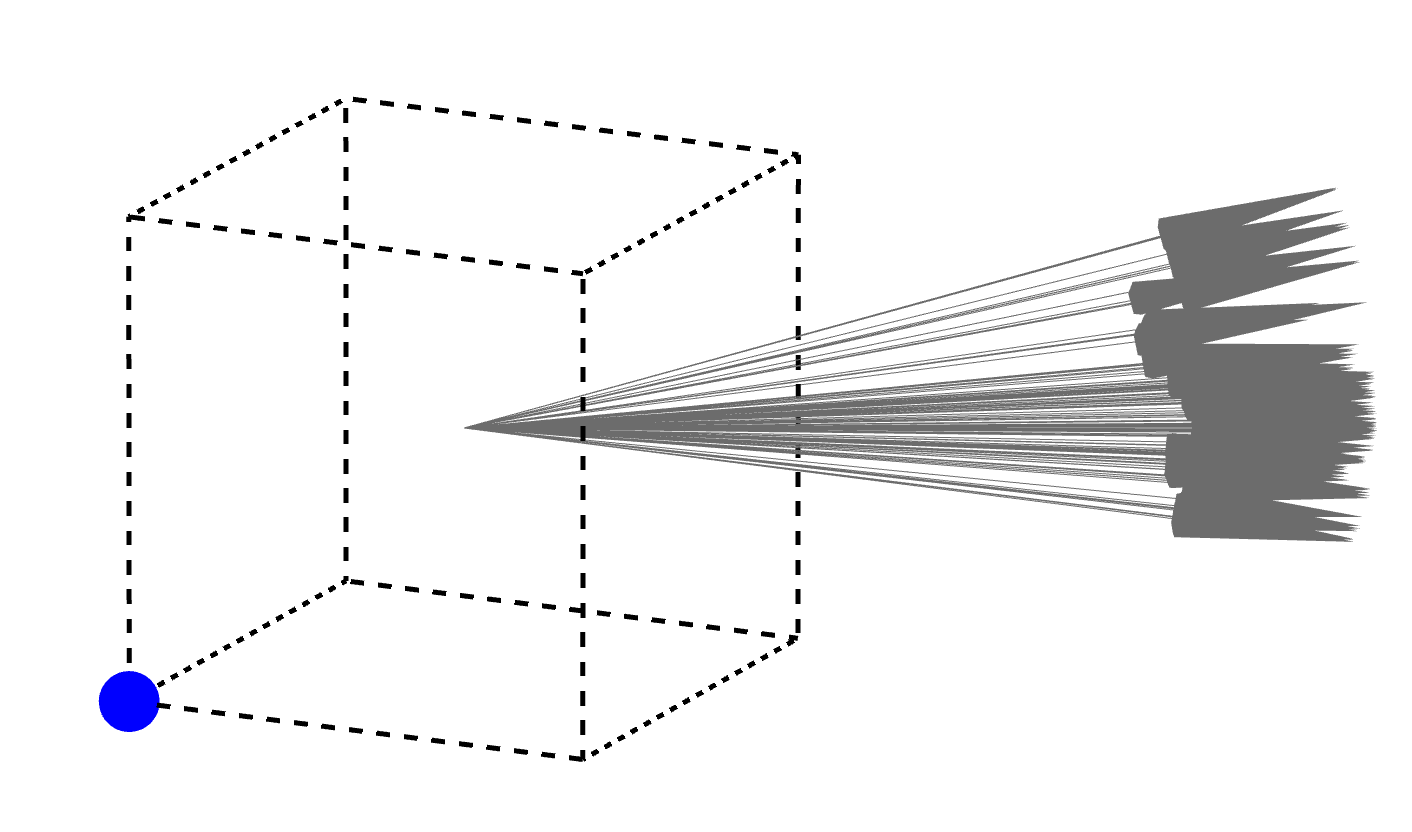
\includegraphics[width=\textwidth]{img/ohne.png}
		\caption{Eine Richtungsbestimmung mit Ausgeschaltetem Clustering\label{fig:ohne}}
	\end{minipage}
	\hfill
	\begin{minipage}[b]{0.45\textwidth}
		\centering
		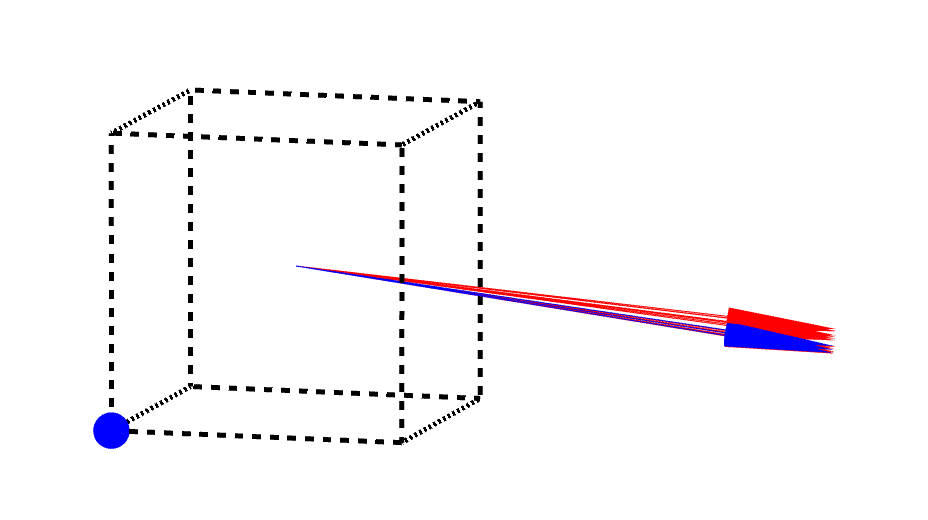
\includegraphics[width=\textwidth]{img/mit.png}
		\caption{Eine Richtungsbestimmung mit Eingeschaltetem Clustering\label{fig:mit}}
	\end{minipage}
\end{figure}